
%
%  $Description: Author guidelines and sample document in LaTeX 2.09$ 
%
%  $Author: ienne $
%  $Date: 1995/09/15 15:20:59 $
%  $Revision: 1.4 $
%

\documentclass[times, 10pt,twocolumn]{article} 
\usepackage{latex8}
\usepackage{times}
\usepackage{graphicx}
\usepackage{epstopdf}

%\documentstyle[times,art10,twocolumn,latex8]{article}

%------------------------------------------------------------------------- 
% take the % away on next line to produce the final camera-ready version 
\pagestyle{empty}

%------------------------------------------------------------------------- 
\begin{document}

\title{Distributed Software Transactional Memory}

\maketitle
\thispagestyle{empty}

\begin{abstract}


   The present paper describes the details of a distributed software
   transactional memory implementation.
   There are 2 scenarios presented for a Master/Server architecture: \\
   a) perfect links and processes (Master and Servers) \\
   b) perfect links and Master, but recoverable Servers \\

   Transaction management, concurrency control, failure detector and 
   replication mechanisms are described for both perfect and fault-tolerant
   architectures.
   
\end{abstract}



%------------------------------------------------------------------------- 
\Section{Introduction}
In the following sections the implementation of a distributed software 
transactional memory library is presented for two scenarios:\\
a) perfect Master, Servers and links\\
b) perfect Master, links and recoverable, sequentially consistent Servers\\

Section \ref{sec:arch} introduces an overview of each scenario. Section 
\ref{sec:algor} discusses the algorithms used for concurrency control, 
transaction management and Client-Server communication


%------------------------------------------------------------------------- 
\Section{Architecture}
\label{sec:arch}

%TODO: Include diagram for both scenarios in different subsections.

%------------------------------------------------------------------------- 
\SubSection{Perfect links and processes}
\label{subsec:perf}
As illustrated in Figure \ref{fig:perf}, the architecture consists of the 
following perfect entities: 
\begin{itemize}
\item {\bf M} - Master server 
\item {\bf S} - Object server
\item {\bf C} - Client      
\end{itemize}

\begin{figure}
\centering
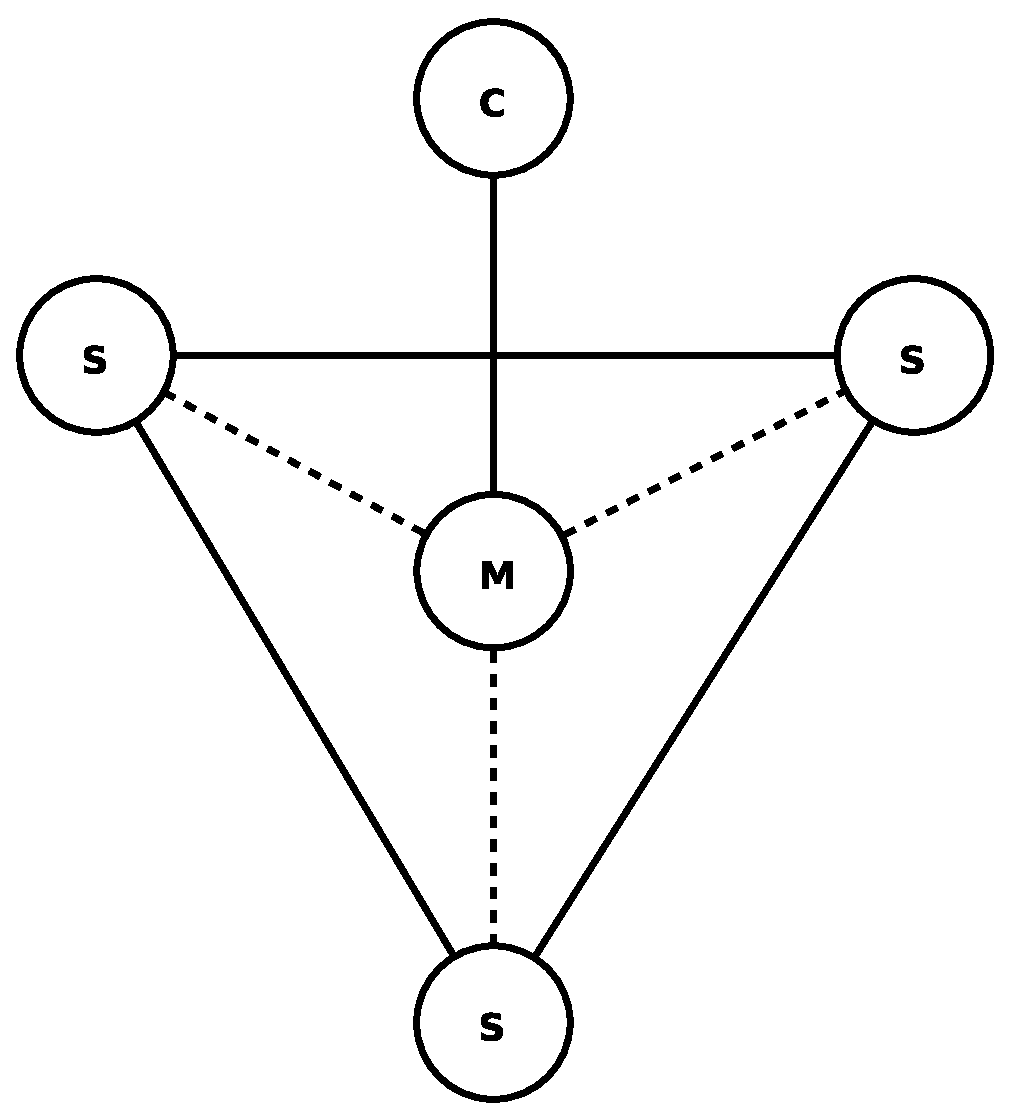
\includegraphics[scale=0.3]{perfect.eps}
\caption{Master/Server entities in a perfect setup}
\label{fig:perf}
\end{figure}

%------------------------------------------------------------------------- 
\SubSection{Recoverable, replicated Servers with perfect Master}
\label{subsec:recov}

%------------------------------------------------------------------------- 
\SubSection{Coordinator/Master responsiblities}
\label{subsec:respon}

The Coordinator's responsabilities and interface is different for the two scenarios (perfect and fault-tolerant) detailed in Section \ref{sec:arch}. For instance, assuming perfect links and non-Byzantine processes, the Coordinator can be any of the Servers, thus balancing the load among the servers. The list of servers the Client chooses from is supplied by the Master to the Client and changes every time the group membership changes (i.e. Servers leave or join). 

%------------------------------------------------------------------------- 
\Section{Algorithms}
\label{sec:algor}

%------------------------------------------------------------------------ 
\SubSection{Communication}
The following communication occurs {\bf before} the client attempts connection 
to the Master node.
\begin{enumerate}
\item Master starts first followed by the Object Server bootstrap
\item During Object Server bootstrap:
\begin{enumerate}
\item Master identifies the Object Servers trying to connect
\item Master assigns a unique name to the Object Servers for later use as a reference
\end{enumerate}
\item Object Servers's heartbeat messages periodically sent to Master
\end{enumerate}

Upon {\bf attempting a transaction} (object storage) the following communication exists between the Client and Master and Object Servers: 

\begin{enumerate}
\item Client connects to the Master and requests a transaction identifier 
\item Master maintains a global transaction sequence and returns a unique transaction identifier (TID) to the Client. Furthermore, a list of healthy Object Servers is also returned to the Client. 
\item Client generates a unique ID (integer) when generating the object and also be used in order to select an available server from the list (used in a modulo function)
\item Client uses the modulo result to connect to the Object Server and store the object representing the tentative versions of the transaction.
\end{enumerate}

When the Client attempts to {\bf manipulate an existing object} in the {\it perfect} Object Servers, the following communication takes place:
\begin{enumerate}
\item Client requests and retrieves TID from Master
\item Client retrieves object's previously generated unique ID
\item Client applies modulo on the retrieved ID to locate the relevant Object Server to request for reference
\item With the retrieved object reference, client can manipulate the object value
\end{enumerate}

%------------------------------------------------------------------------- 
\SubSection{Transaction Management and Concurrency Control}
\label{subsec:transmgt}
The {\it Flat Transaction} model allows for a client to manipulate objects on multiple servers in a single transaction. With regards to concurrency control {\it Timestamp Ordering} is being chosen. Figure \ref{fig:flat} illustrates a flat transaction model setup with a {\it transaction} being executed from the client on 3 servers.

\begin{figure}
\centering
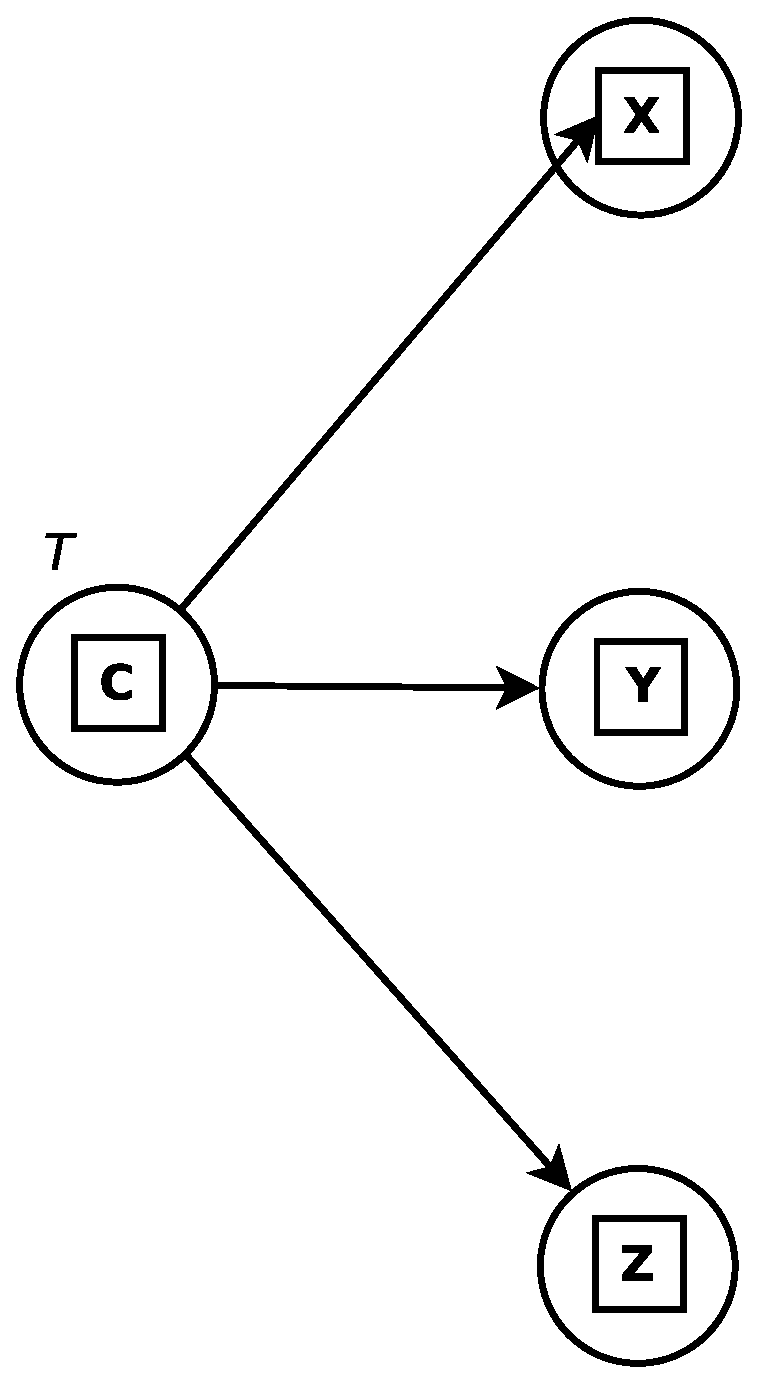
\includegraphics[scale=0.2]{flat-transaction.eps}
\caption{Flat Transaction model between a Client and 3 Servers}
\label{fig:flat}
\end{figure}


The advantages of choosing {\it Timestamp Ordering} over {\it Two-Phase Locking} or {\it Optimistic Concurrency} options are the following: 
\begin{itemize}
\item Deadlock prevention - common with the use of locks
\item Better performance for transactions with predominantly {\it read} operations \cite{bernstein1987concurrency}
\item Faster conflict resolution when compared to locking - transactions are aborted immediately. 
\end{itemize}

The following steps are made when performing a transaction in the {\bf perfect} environment - assuming no link or process failures: 
\begin{enumerate}
\item Client acquires transaction ID from the Master
\item Client passes TID to the Object Server
\item Object Server calls the Coordinator's(Master's) {\it join()} method along with TID as parameter
\item Client manipulates objects directly on the Object Server
\item Upon transaction end, Client asks the Coordinator to either {\it Abort} or {\it Commit} 
\item Coordinator will request a each participant server in the transaction to indicate whther it can commit a transaction or not.
\item If all participants answer {\it yes}, Coordinator issues {\bf doCommit(TID)} command such that each parcipant commits its part of the transaction
\item Once completed, all servers acknowledge the commit and Coordinator notifies the Client that it's successful.
\item Should any of the participant servers be unable or disagree to commit and aborts, the Coordinator will request all the remaining participants to abort. Client will then be notified.
\end{enumerate}

%------------------------------------------------------------------------- 
\Section{Footnotes}

Please use footnotes sparingly%
\footnote
   {%
     Or, better still, try to avoid footnotes altogether.  To help your 
     readers, avoid using footnotes altogether and include necessary 
     peripheral observations in the text (within parentheses, if you 
     prefer, as in this sentence).
   }
and place them at the bottom of the column on the page on which they are 
referenced. Use Times 8-point type, single-spaced.


%------------------------------------------------------------------------- 
\SubSection{References}

%------------------------------------------------------------------------- 
\SubSection{Conclusions}

%------------------------------------------------------------------------- 
\bibliographystyle{latex8}
\bibliography{latex8}

\end{document}

